\documentclass[11.5pt]{article}
\usepackage[utf8]{inputenc}
\usepackage[T1]{fontenc}
\usepackage[textwidth = 460pt,top = 80pt, bottom = 80pt]{geometry}
\usepackage{graphicx}
\usepackage[justification=default]{subfig} %Manage sub-figures 
\usepackage[update]{epstopdf}
\usepackage[labelfont=bf]{caption}
\usepackage[dvipsnames]{xcolor}
\usepackage{fancyhdr}
\usepackage{booktabs}
\usepackage{multicol}
\usepackage{multirow}
\usepackage{titling}
\usepackage{float}
\usepackage{bm}
\usepackage[intlimits]{empheq}
\usepackage[hidelinks]{hyperref}
\usepackage{amsmath}


%Bibliography

\usepackage{csquotes}
\usepackage[sorting=none,%
sortcites=true,%
bibencoding=ascii,%
autopunct=true,%
hyperref=true,%
language=auto,%
%backref=true,%
url=false,%
%maxcitenames=10,%
%minbibnames = 20,%
maxbibnames = 3,%
giveninits, 
natbib = false,
isbn=false,%
backend=biber]{biblatex}
\addbibresource{bibliography.bib}

\usepackage[]{hyperref}
\usepackage{cleveref}
%%% CREF setup
\crefname{equation}{Eq.}{Eqs.}
\crefname{table}{Table}{Tables}
\crefname{figure}{Fig.}{Figs.}


\begin{document}

\begin{titlingpage}
    \begin{center}
        \begin{figure}
            \centering
            
\includegraphics[width=0.6\textwidth]{graphics/logopolimi_mod.jpg}
        \end{figure}
        \Large{\textsc{Politecnico di Milano \\ School of Industrial and Information Engineering \\ M.Sc. in High Performance Computing}}

        \vspace{1cm}

        \rule{0.95\textwidth}{0.7mm}
        {\Large{\textbf{Final project: \\Classify musical genre using audio files}}}
        \rule{0.95\textwidth}{0.7mm}

        \vspace{1cm}

        \large{Prof. Edie Miglio \\ A.Y. 2024-2025}

        \vspace{1cm}

        \large{Authors: \\ \textbf{Peng Rao} (ID 270661)}
    \end{center}

\end{titlingpage}

\pagenumbering{roman}

\tableofcontents

\clearpage

\setcounter{page}{1}
\pagenumbering{arabic}

\section{Introduction} \label{sec:introduction}
In today's fast-paced world, with millions of new songs released daily, organizing music into genres is essential for improving user experiences on streaming platforms and managing music libraries efficiently. However, manually classifying songs by genre is a time-consuming task. This is where \textbf{machine learning} offers a powerful solution.

\section{Data Exploration} \label{sec:data_exploration}
\subsection{Data Description}
The \textbf{GTZAN dataset} is the most-used public dataset for evaluation in machine listening research for music genre recognition (MGR). The files were collected in 2000-2001 from a variety of sources including personal CDs, radio, microphone recordings, in order to represent a variety of recording conditions.\cite{GTZANDatasetMusic}

The dataset consists of 1000 audio tracks each 30 seconds long. It contains 10 genres, each represented by 100 tracks. The tracks are all 22050Hz Mono 16-bit audio files in .wav format. The features of the dataset can be summarized as follows table \ref{tab:dataset}.
\begin{table}[h]
    \centering
    \begin{tabular}{cccccc}
        \toprule
        \textbf{Category} & \textbf{Feature}                                     & \textbf{Description}                 \\
        \midrule
        General           & filename, length, label                              & File metadata and classification     \\
        Spectral          & chroma\_stft, rms, spectral\_centroid, rolloff, etc. & Frequency-based characteristics      \\
        Harmonic          & harmony, perceptr, tempo                             & Harmonic and perceptual content      \\

        MFCCs             & mfcc1-20 (mean, var)                                 & Captures timbral properties of audio \\

        \bottomrule
    \end{tabular}
    \caption{GTZAN Dataset Features}
    \label{tab:dataset}
\end{table}

\subsection{Waveform Analysis}
The waveform of an audio signal is a representation of the amplitude of the sound wave as a function of time. I visualized the waveform of a sample track in figure \ref{fig:waveform}. The waveform figures show that some genres, like pop, metal, and hip-hop, exhibit high amplitude variations throughout the track. Others, like classical and jazz, show more varied amplitude patterns, reflecting their dynamic nature. Blues and reggae have distinct waveform structures that differentiate them from other genres.
\begin{figure}[H]
    \centering
    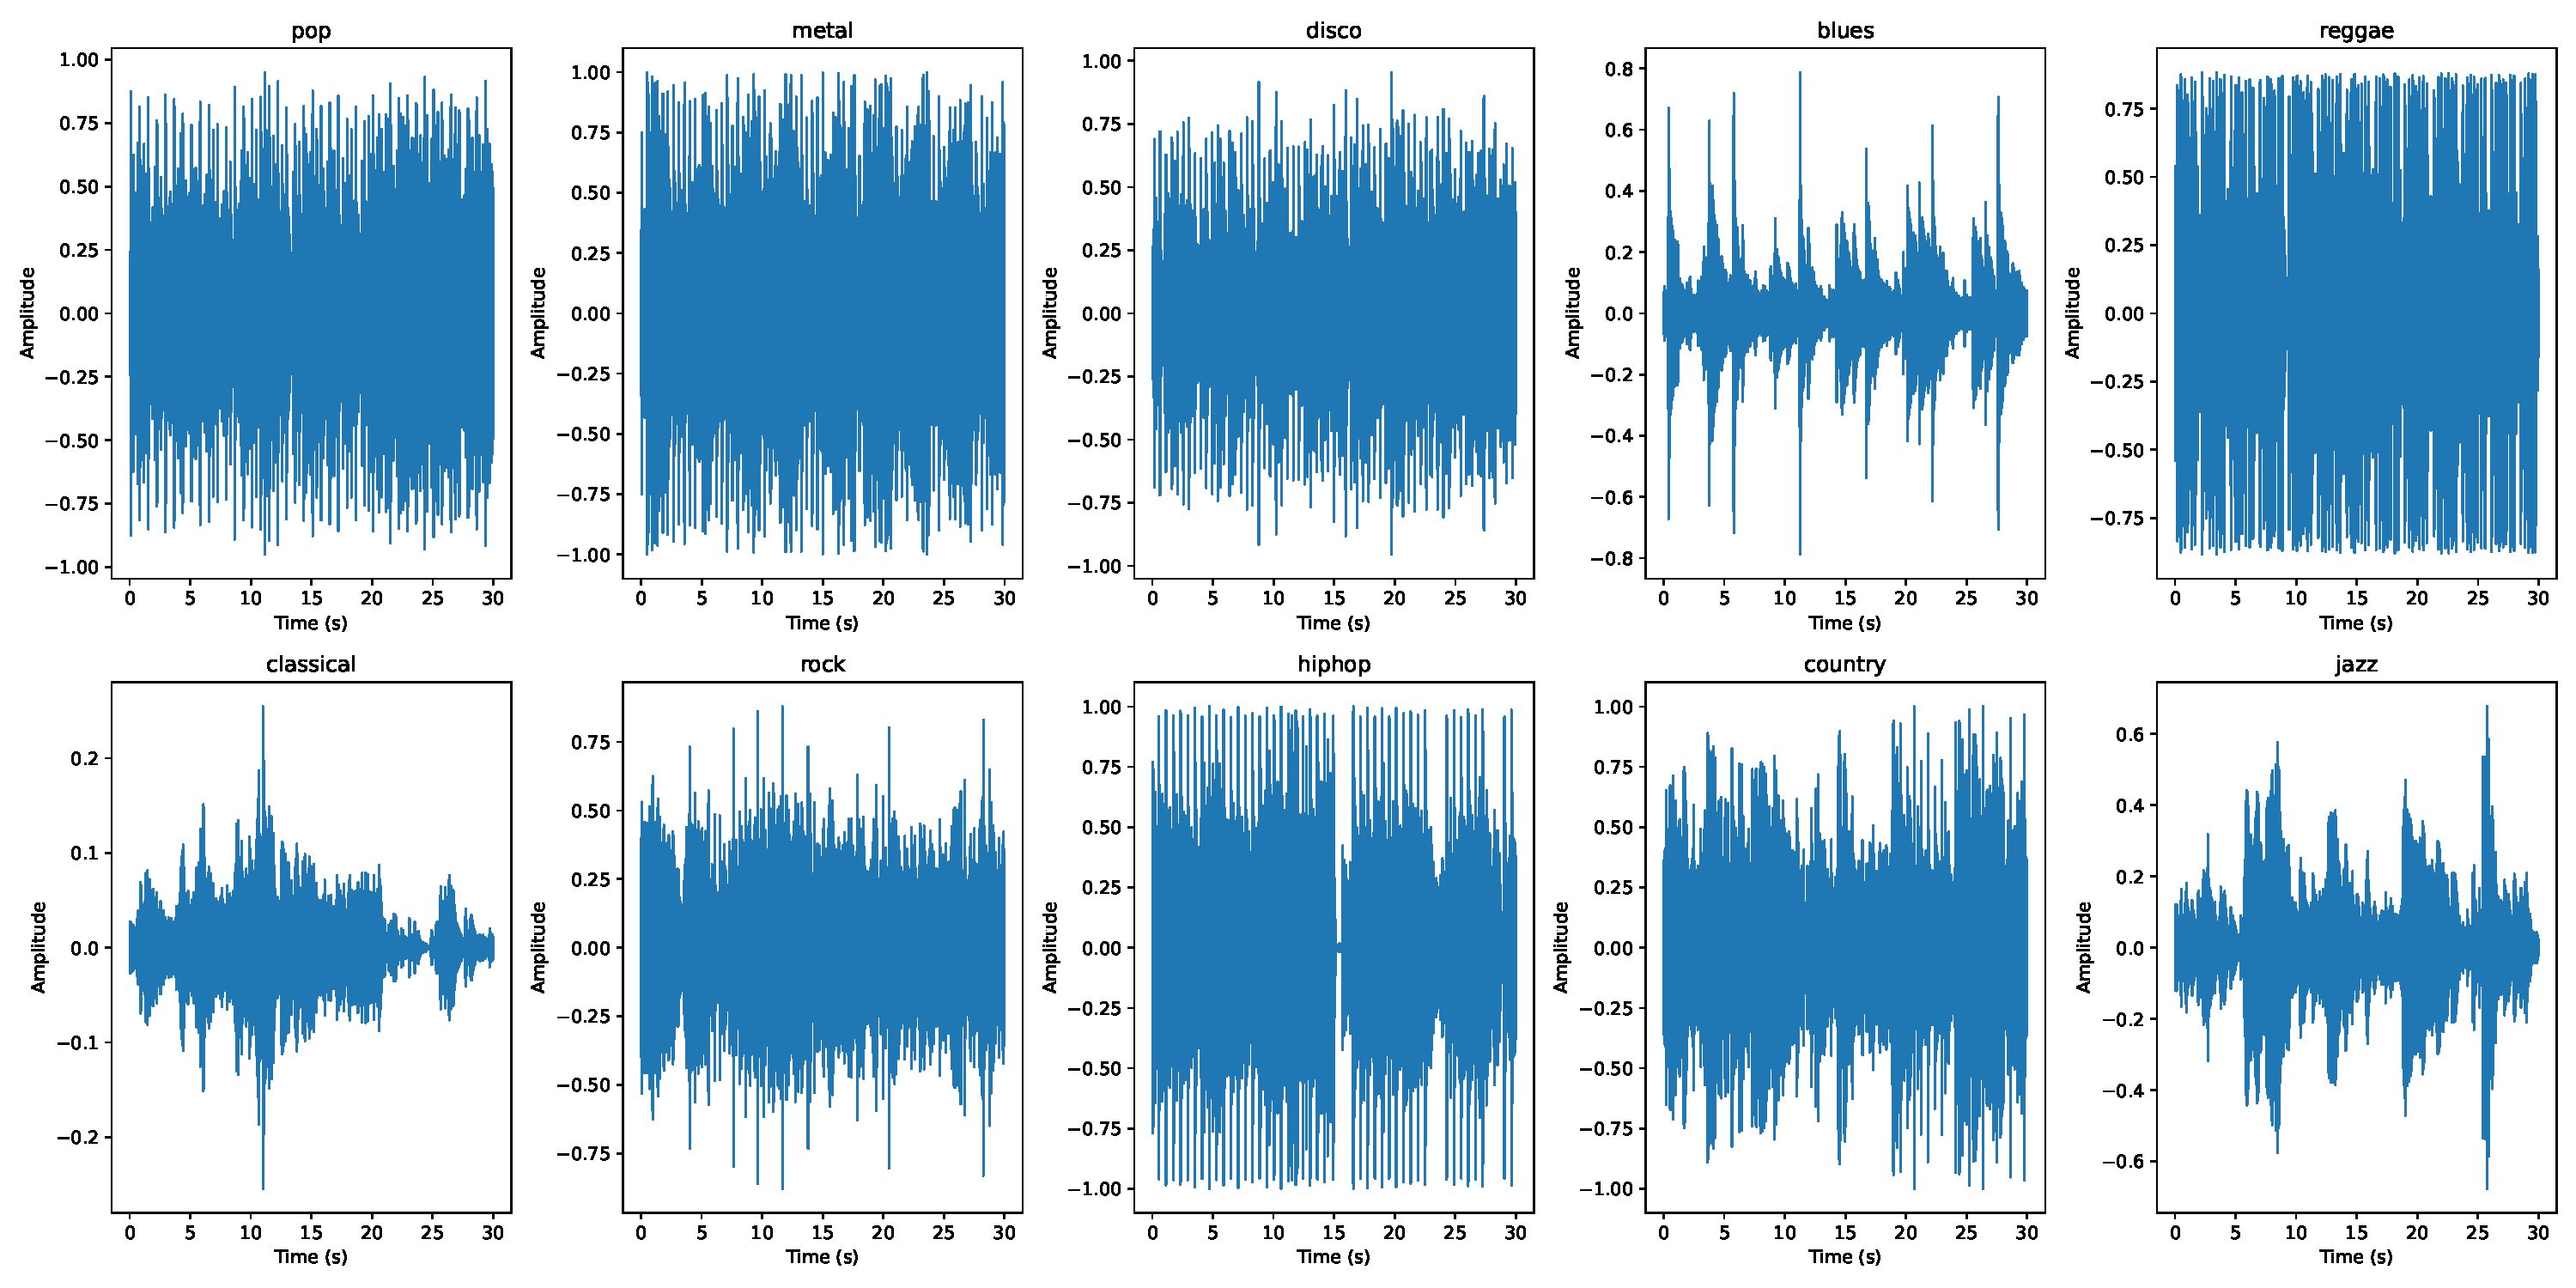
\includegraphics[width=0.9\textwidth]{graphics/waveform.pdf}
    \caption{Waveform of various sample audios track over time}
    \label{fig:waveform}
\end{figure}

\subsection{Chroma Analysis}
Chroma features (or chroma vectors) are audio features used in music information retrieval to represent the harmonic and tonal content of an audio signal. They capture the distribution of energy across the 12 different pitch classes (e.g., C, C\#, D, D\#, ..., B) regardless of octave. I visualized the changes in chroma features over time for a sample track in figure \ref{fig:chroma}. Each row corresponds to one pitch class, showing how much energy is present in that pitch class over time. Genres like rock, blues, pop, and hip-hop show dense chroma activity, indicating frequent chord changes. Classical and jazz have more structured patterns (jazz is showing more harmonic complexity).
\begin{figure}[h]
    \centering
    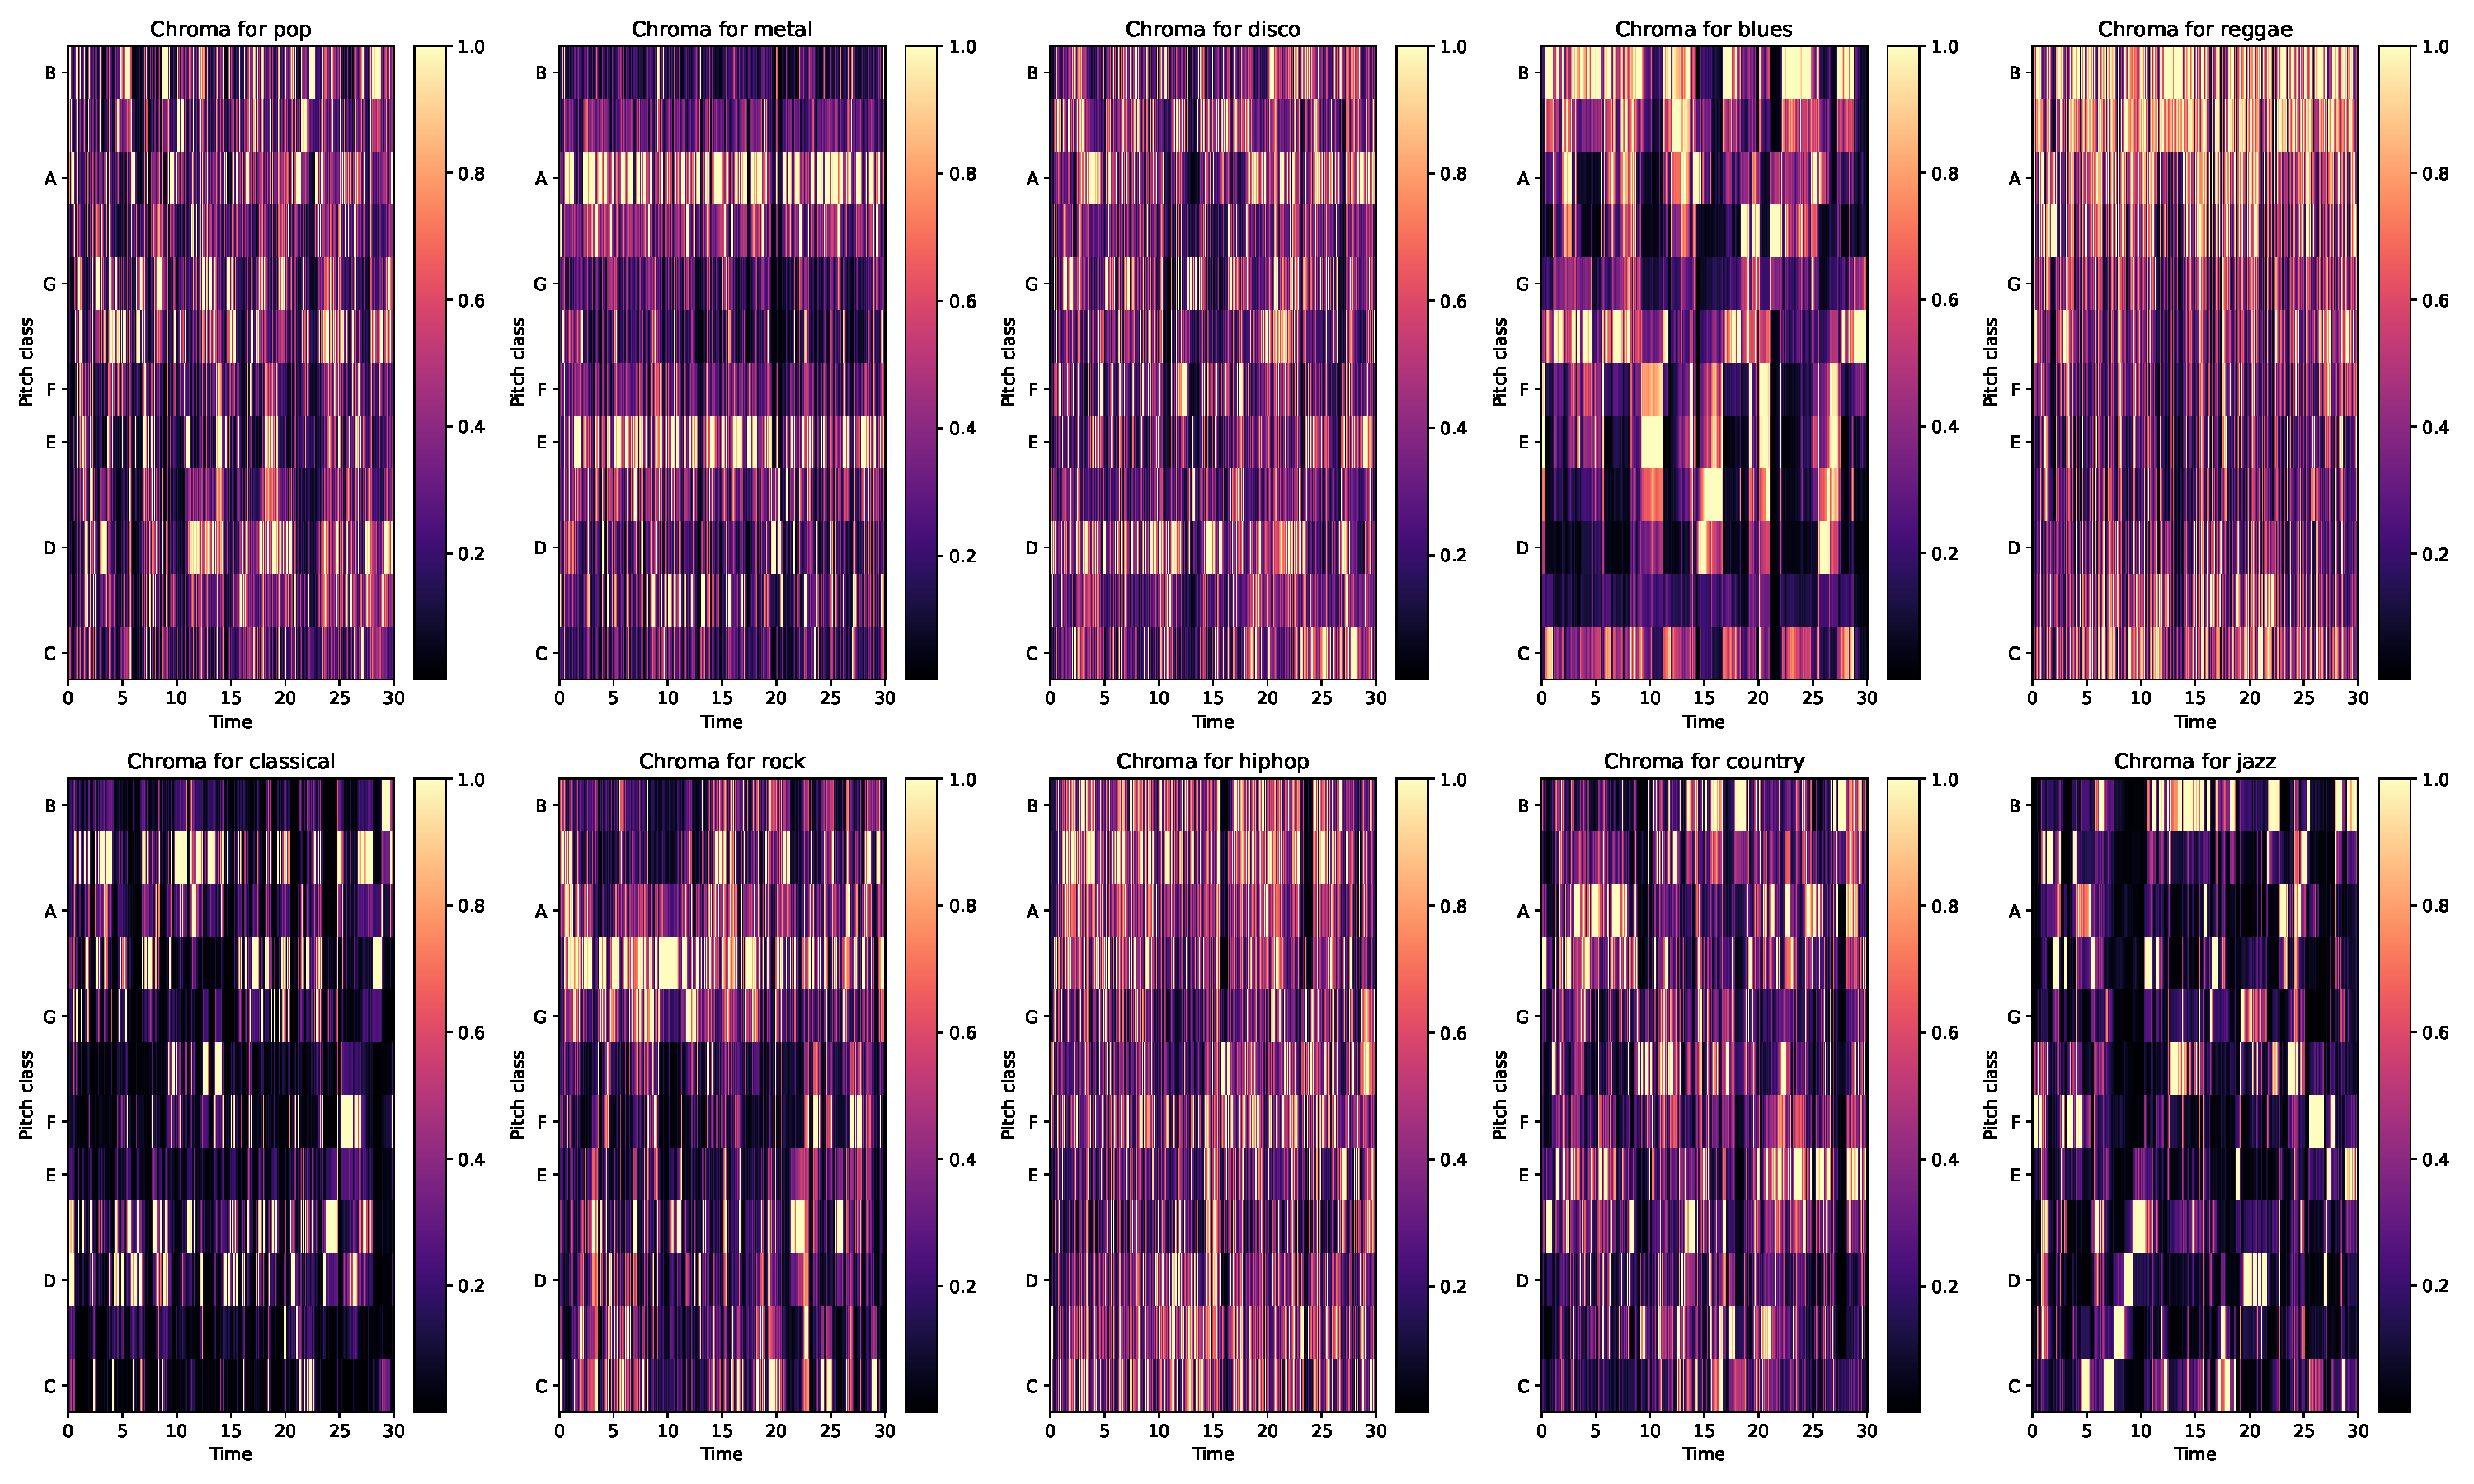
\includegraphics[width=0.9\textwidth]{graphics/chroma.pdf}
    \caption{Chroma Features of various pitch classes over time}
    \label{fig:chroma}
\end{figure}

\subsection{MFCC Analysis}
MFCC is a feature extraction technique commonly used in speech and audio processing. It transforms a raw audio signal into a compact, perceptually relevant representation by mimicking the human auditory system. Typically, the first 13-20 coefficients are used as features. I visualized the MFCCs of a sample track in figure \ref{fig:mfcc}. The MFCCs capture the timbral properties of the audio signal, showing how the spectral content changes over time. Genres like rock, blues, and pop exhibit high variability in MFCCs, reflecting their diverse timbral characteristics. Classical and jazz have more structured patterns, indicating more consistent timbral properties.
\begin{figure}[h]
    \centering
    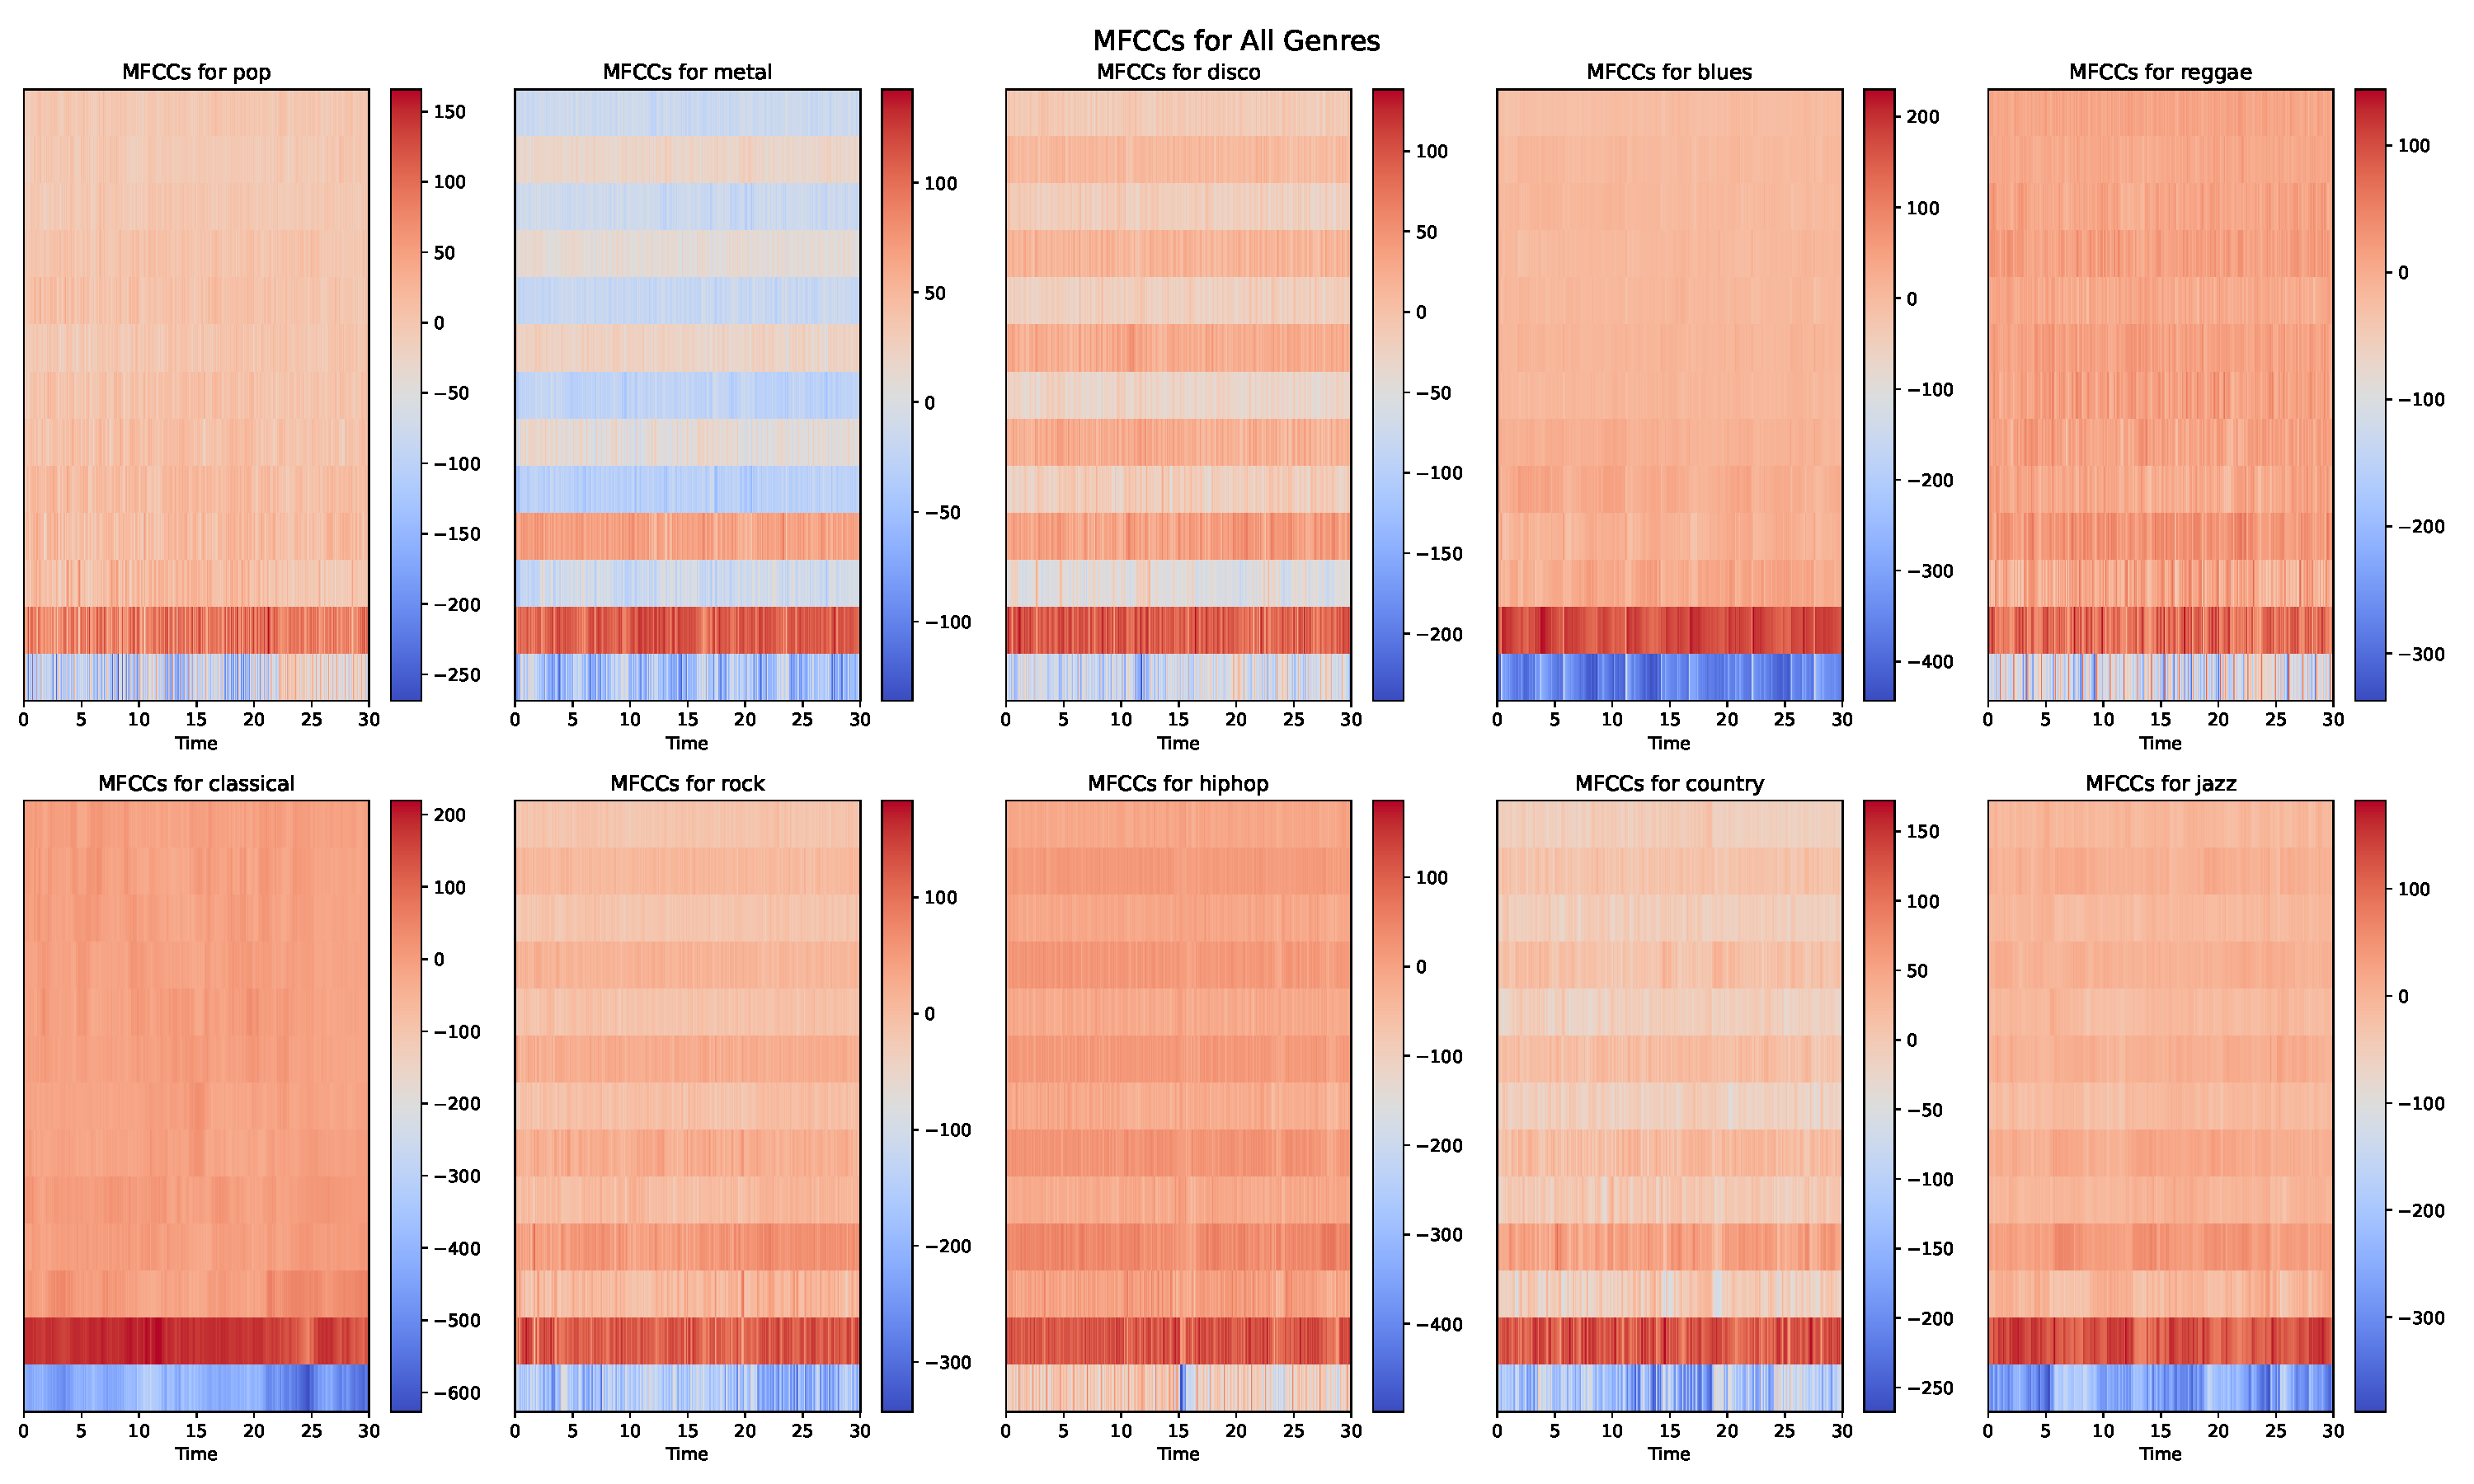
\includegraphics[width=0.9\textwidth]{graphics/mfccs.pdf}
    \caption{MFCC13 of various sample audios track over time}
    \label{fig:mfcc}
\end{figure}

\subsection{Principal Component Analysis}
Principal Component Analysis (PCA) is a dimensionality reduction technique that transforms data into a lower-dimensional space while preserving as much variance as possible. I applied PCA to the dataset and visualized the first two principal components in figure \ref{fig:pca}.
\begin{figure}[H]
    \centering
    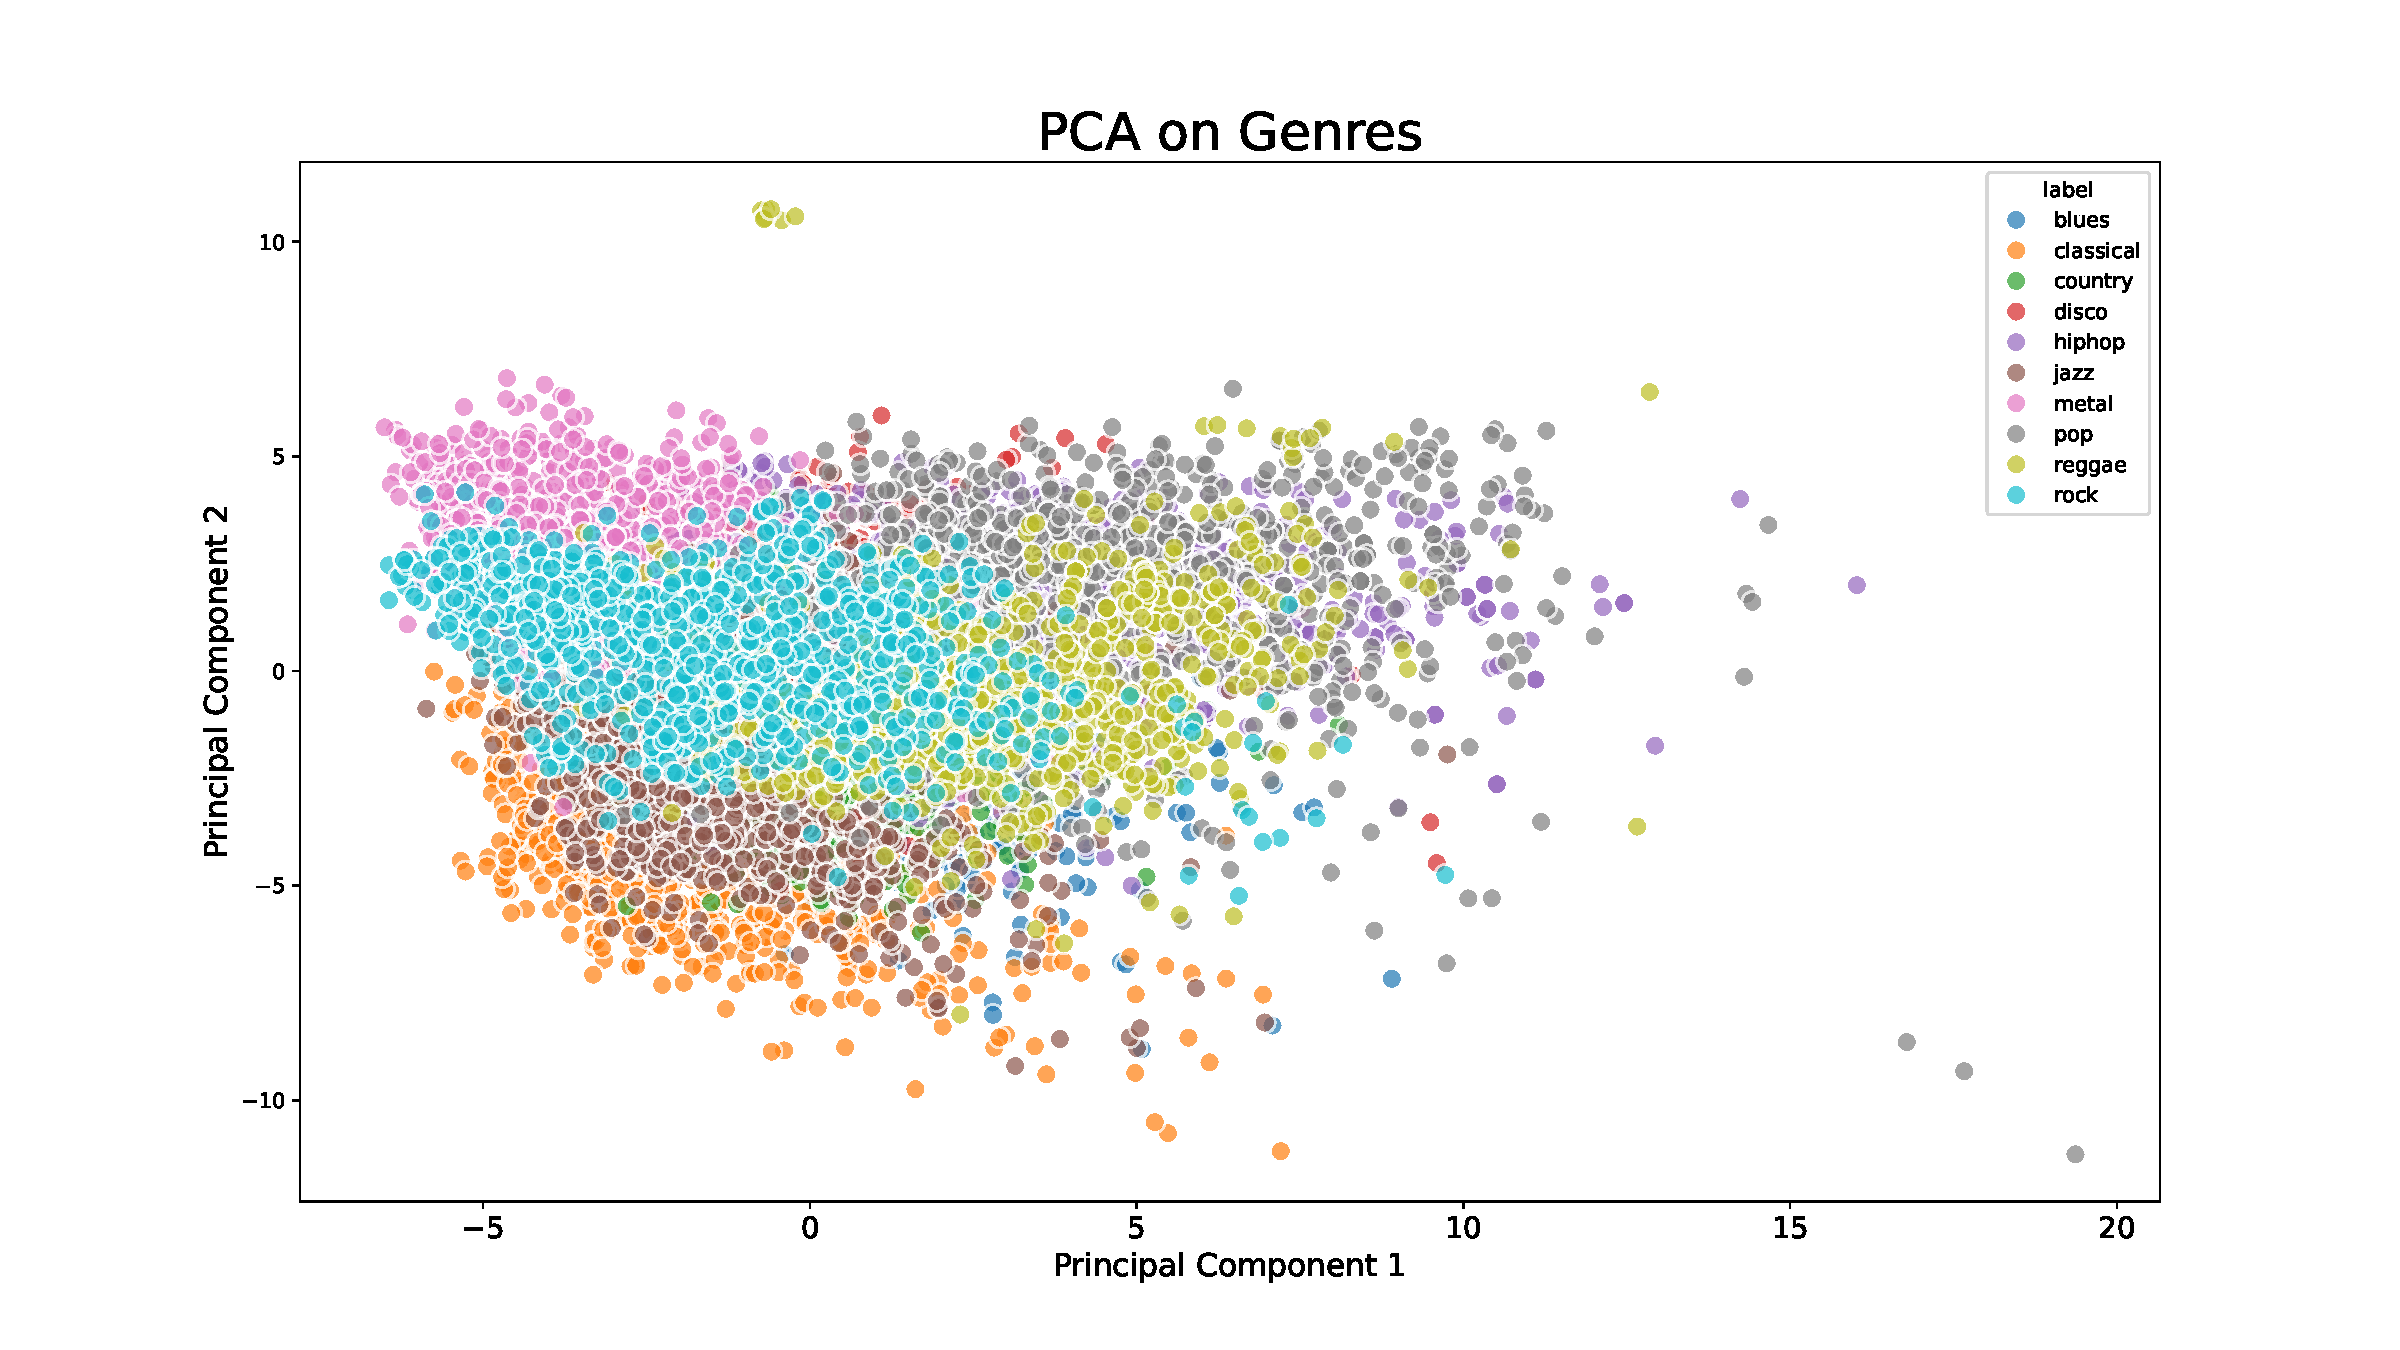
\includegraphics[width=0.9\textwidth]{graphics/pca.pdf}
    \caption{PCA of the GTZAN dataset}
    \label{fig:pca}
\end{figure}
b
\section{Data Preprocessing} \label{sec:data_preprocessing}
\subsection{Normalization}
I normalized the dataset to ensure that all features have a similar scale. I used the Min-Max scaling technique to scale the features:
\begin{equation}
    X_{\text{scaled}} = \frac{X - X_{\text{min}}}{X_{\text{max}} - X_{\text{min}}}
\end{equation}

\subsection{Train/Test Split} \label{sec:train_test_split}
I split the dataset into training and testing sets using an 80/20 split. I used the training set to train the model and the testing set to evaluate its performance. The validation has been used during the training phase of the classifers to find good values of the hyperparameters.

\subsection{Cross-Validation Split} \label{sec:cross_validation_split}
I used a 5-fold cross-validation split to evaluate the model's performance. Cross-validation is a technique used to assess the model's generalization performance by training and testing the model on different subsets of the data, as shown in figure \ref{fig:cross_validation}.
\begin{figure}[H]
    \centering
    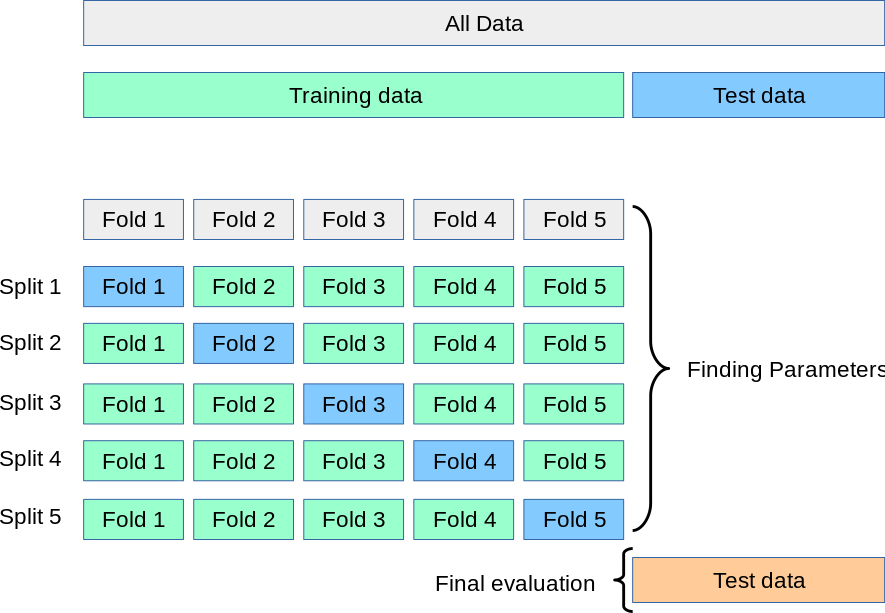
\includegraphics[width=0.5\textwidth]{graphics/grid_search_cross_validation.png}
    \caption{5-fold Cross-Validation Split\cite{31CrossvalidationEvaluating}}
    \label{fig:cross_validation}
\end{figure}

\section{Traditional Machine Learning Models} \label{sec:traditional_ml}
\subsection{Baseline Models}
I trained several traditional machine learning models on the dataset to establish a baseline performance. The models I used are:
\begin{itemize}
    \item \textbf{Logistic Regression}
    \item \textbf{Support Vector Machine}
    \item \textbf{Decision Tree}
    \item \textbf{Random Forest}
    \item \textbf{XGBoost}
\end{itemize}
The models were trained using the default hyperparameters and evaluated using cross-validation. The results of training set are summarized in figure \ref{fig:baseline_models}.
\begin{figure}[H]
    \centering
    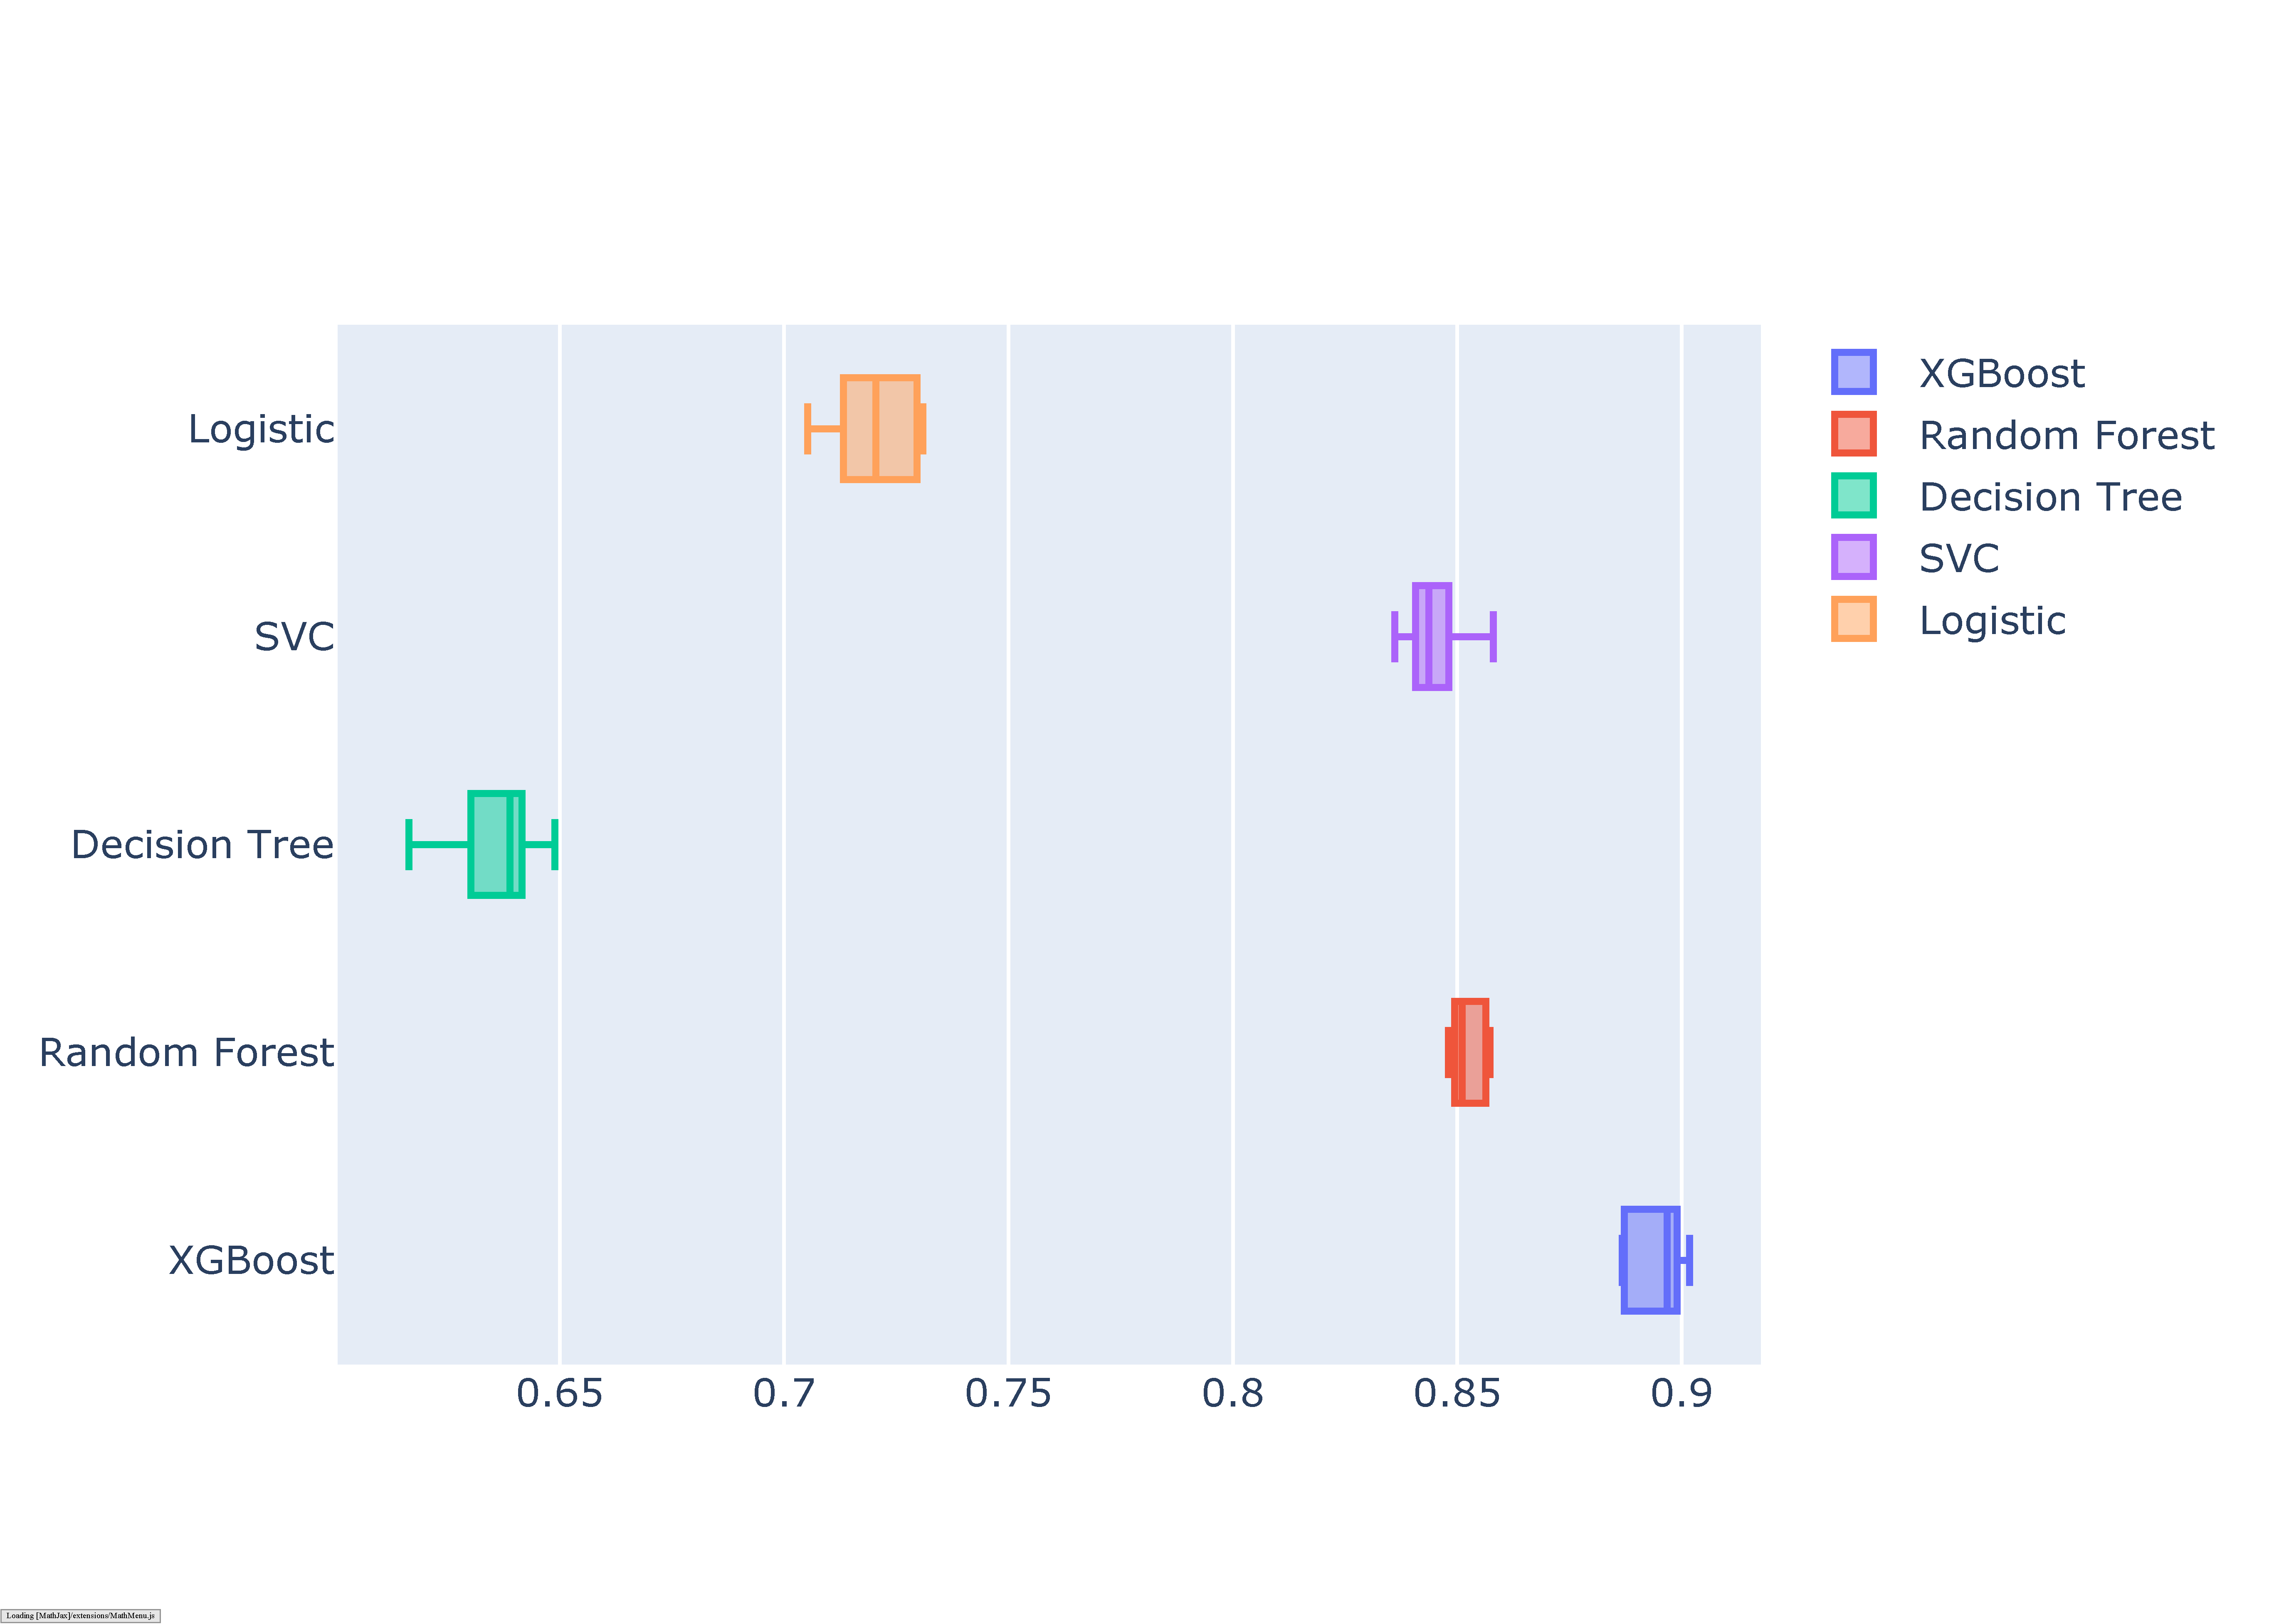
\includegraphics[width=0.9\textwidth]{graphics/baseline_models.pdf}
    \caption{Baseline Models Performance on training set}
    \label{fig:baseline_models}
\end{figure}

\subsection{Model Evaluation}
I evaluated the Xgboost model on the testing set and obtained an accuracy of 0.75. The confusion matrix shows that the model performs well for some genres (e.g., classical, jazz) but struggles with others (e.g., metal, hip-hop). The model's precision, recall, and F1-score are summarized in figure \ref{fig:xgboost_evaluation}.
\begin{figure}[H]
    \centering
    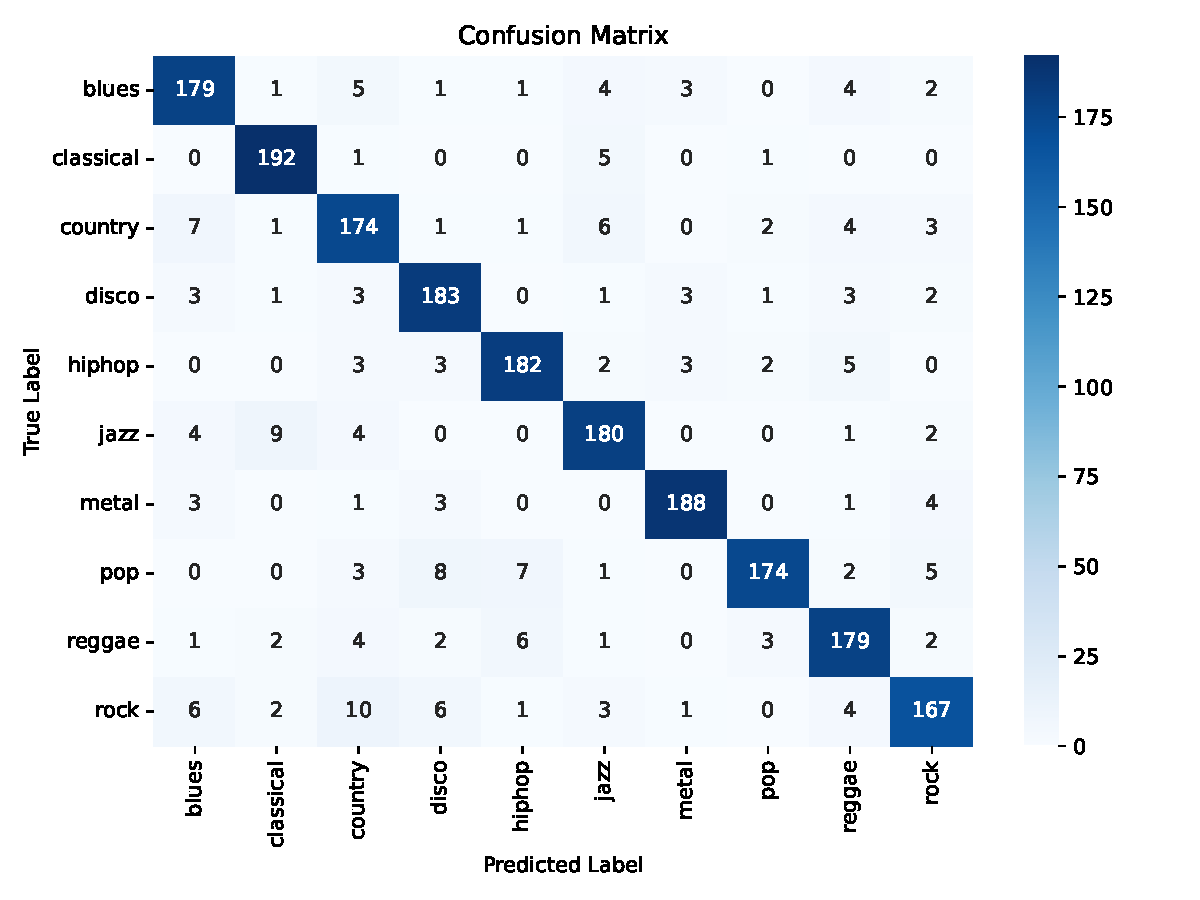
\includegraphics[width=0.9\textwidth]{graphics/confusion_matrix.pdf}
    \caption{XGBoost Model Evaluation on testing set}
    \label{fig:xgboost_evaluation}
\end{figure}

\subsection{Hyperparameter Tuning}
I used RandomizedSearchCV to tune the hyperparameters of the XGBoost model. I performed a randomized search over a predefined hyperparameter grid and selected the best hyperparameters based on the model's performance. The hyperparameters I tuned were:
\begin{itemize}
    \item \textbf{max\_depth}: Maximum depth of the tree
    \item \textbf{learning\_rate}: Step size shrinkage used in update to prevent overfitting
    \item \textbf{n\_estimators}: Number of boosting rounds
    \item \textbf{subsample}: Subsample ratio of the training instances
    \item \textbf{colsample\_bytree}: Subsample ratio of columns when constructing each tree
\end{itemize}
The best hyperparameters found by RandomizedSearchCV were:
\begin{itemize}
    \item \textbf{max\_depth}: 6
    \item \textbf{learning\_rate}: 0.1
    \item \textbf{n\_estimators}: 100
    \item \textbf{subsample}: 0.8
    \item \textbf{colsample\_bytree}: 0.8
    \item \textbf{objective}: 'multi:softmax'
\end{itemize}

\section{Convolutional Neural Network (CNN)} \label{sec:cnn}
\section{Conclusion} \label{sec:conclusion}

\clearpage
\printbibliography[heading=bibintoc, title = {References}]
\end{document}